\section{Transaction process screenshots}\label{sec:appendix-screenshots}

% //ADD Screensoht descriptions

    \centerline{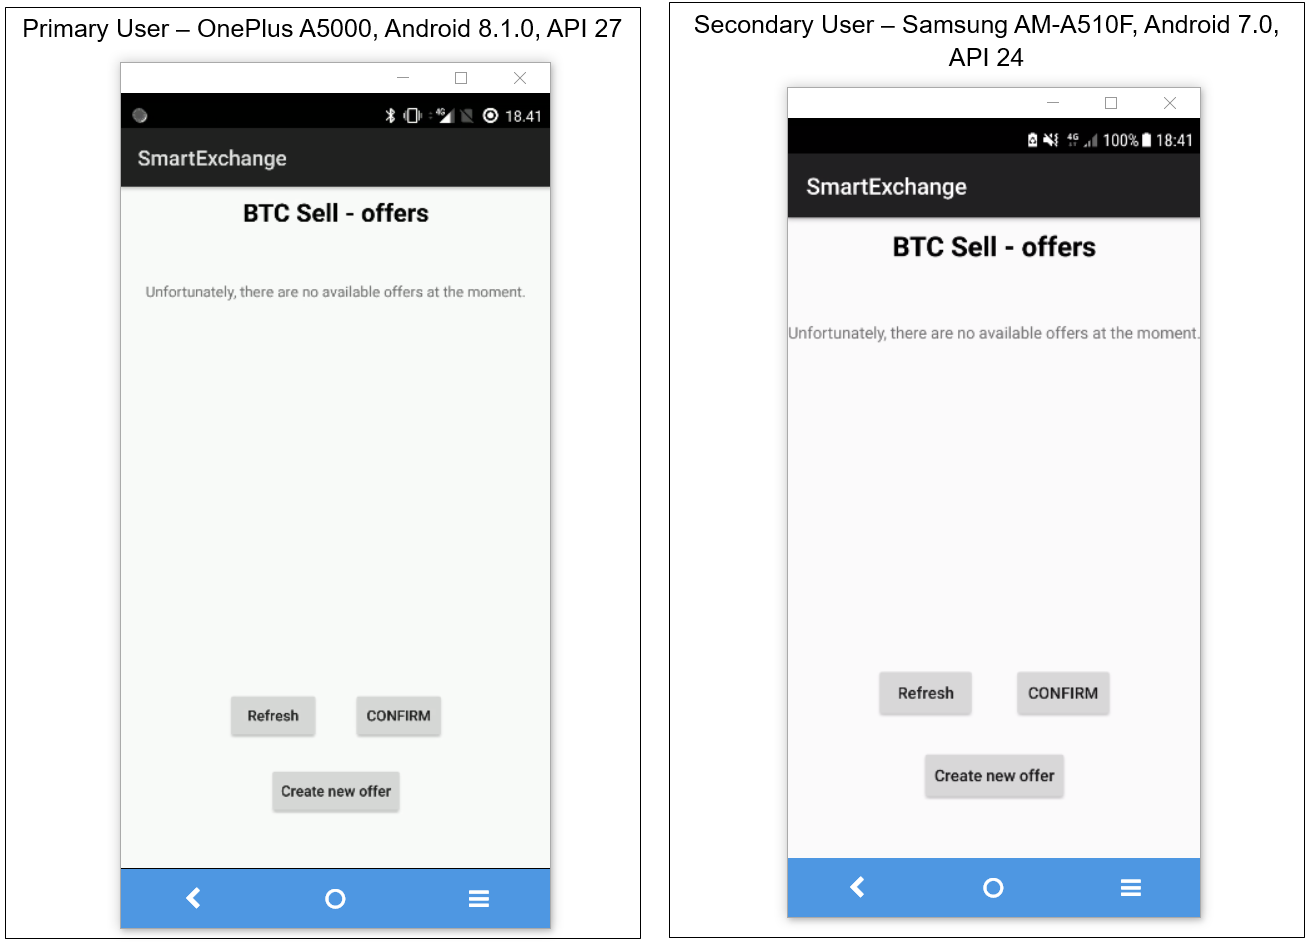
\includegraphics[width=0.75\textwidth]{screenshots/screen020}}
    \centerline{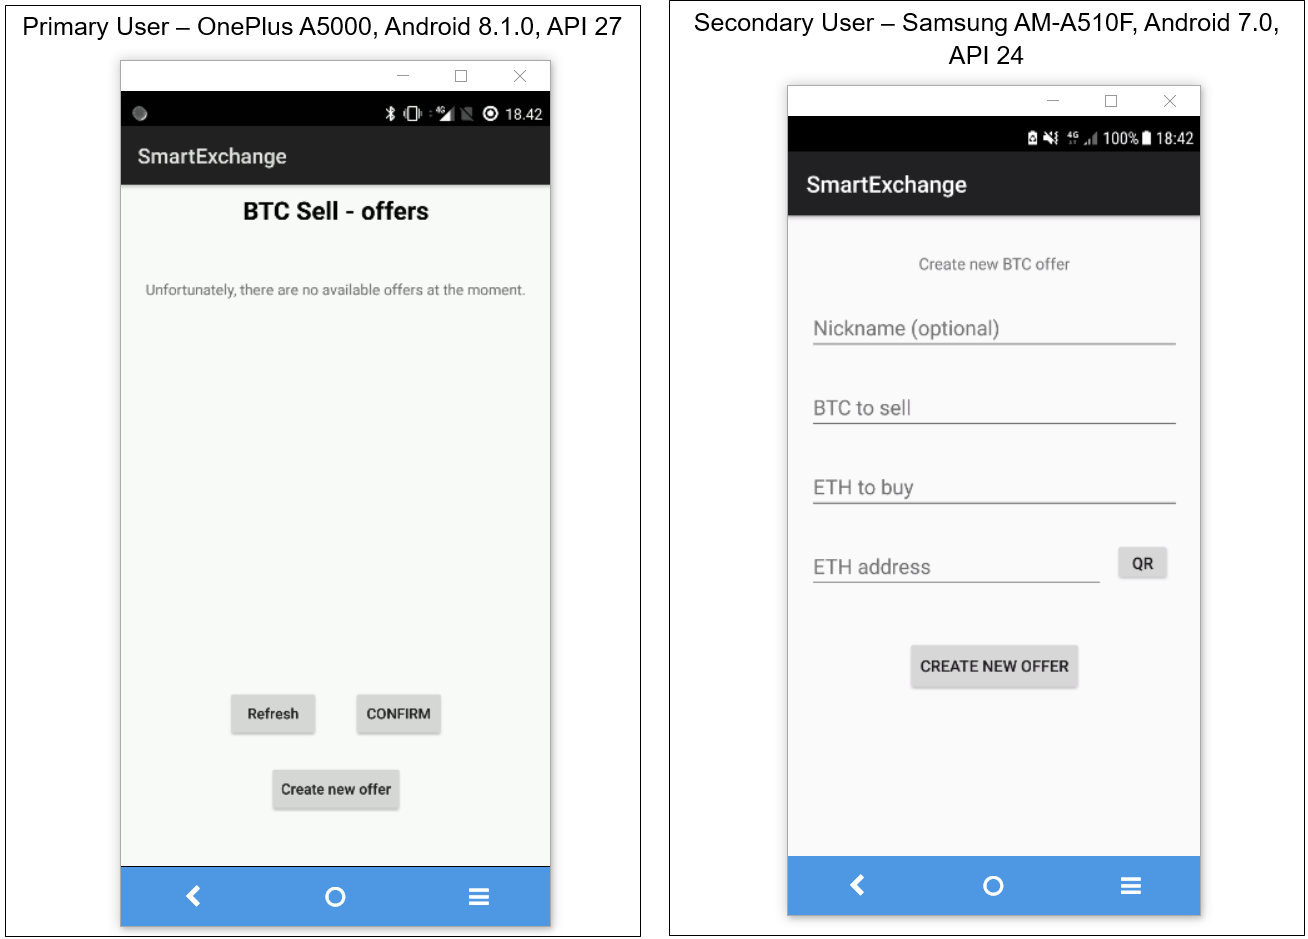
\includegraphics[width=0.75\textwidth]{screenshots/screen031}}
    \textit{Top:}    Front page of the application\\
    \textit{Bottom:} The secondary user clicked on \textit{Create new offer}.\\
    \centerline{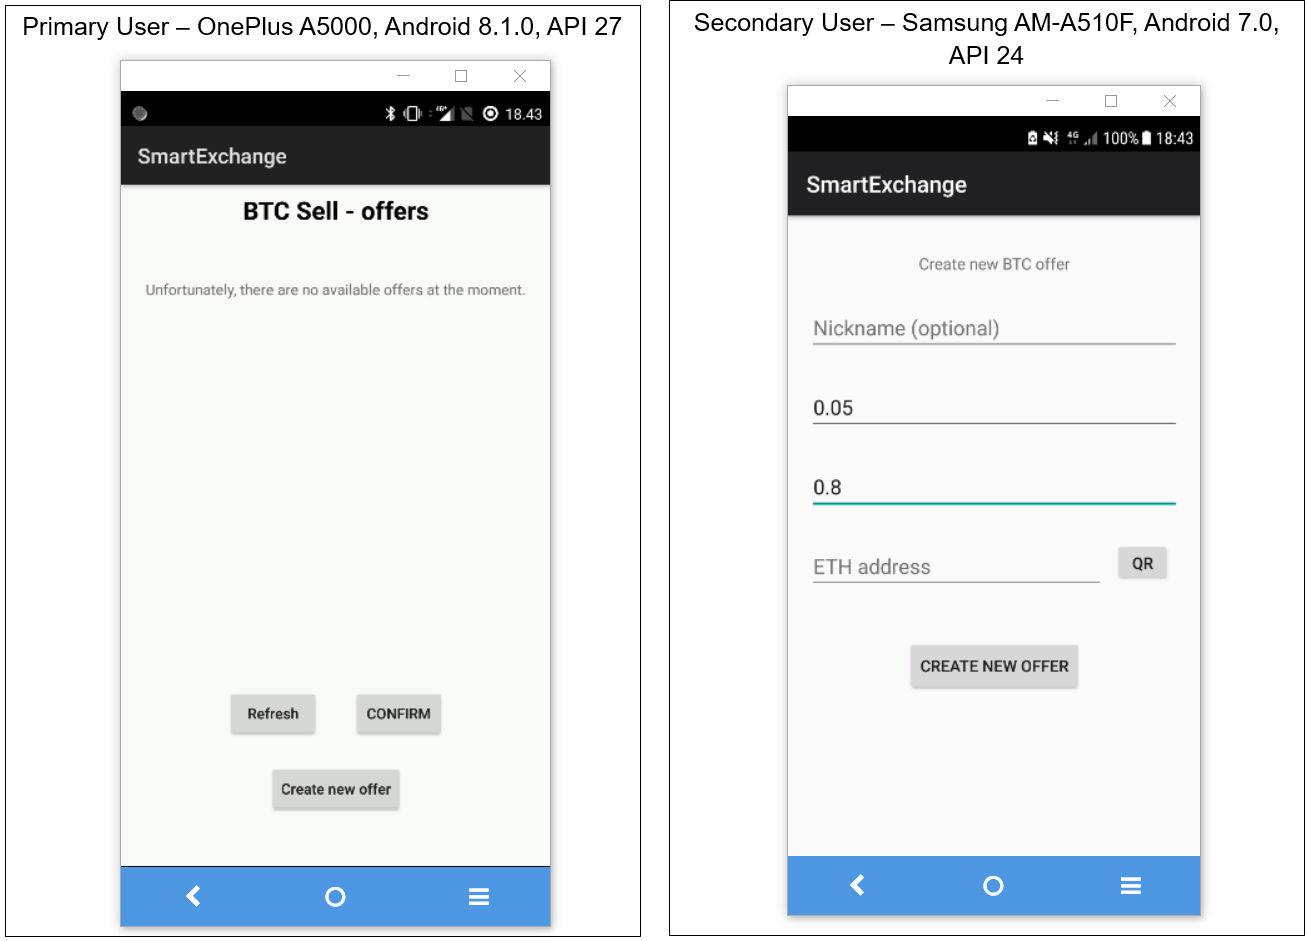
\includegraphics[width=0.85\textwidth]{screenshots/screen032}}
    \centerline{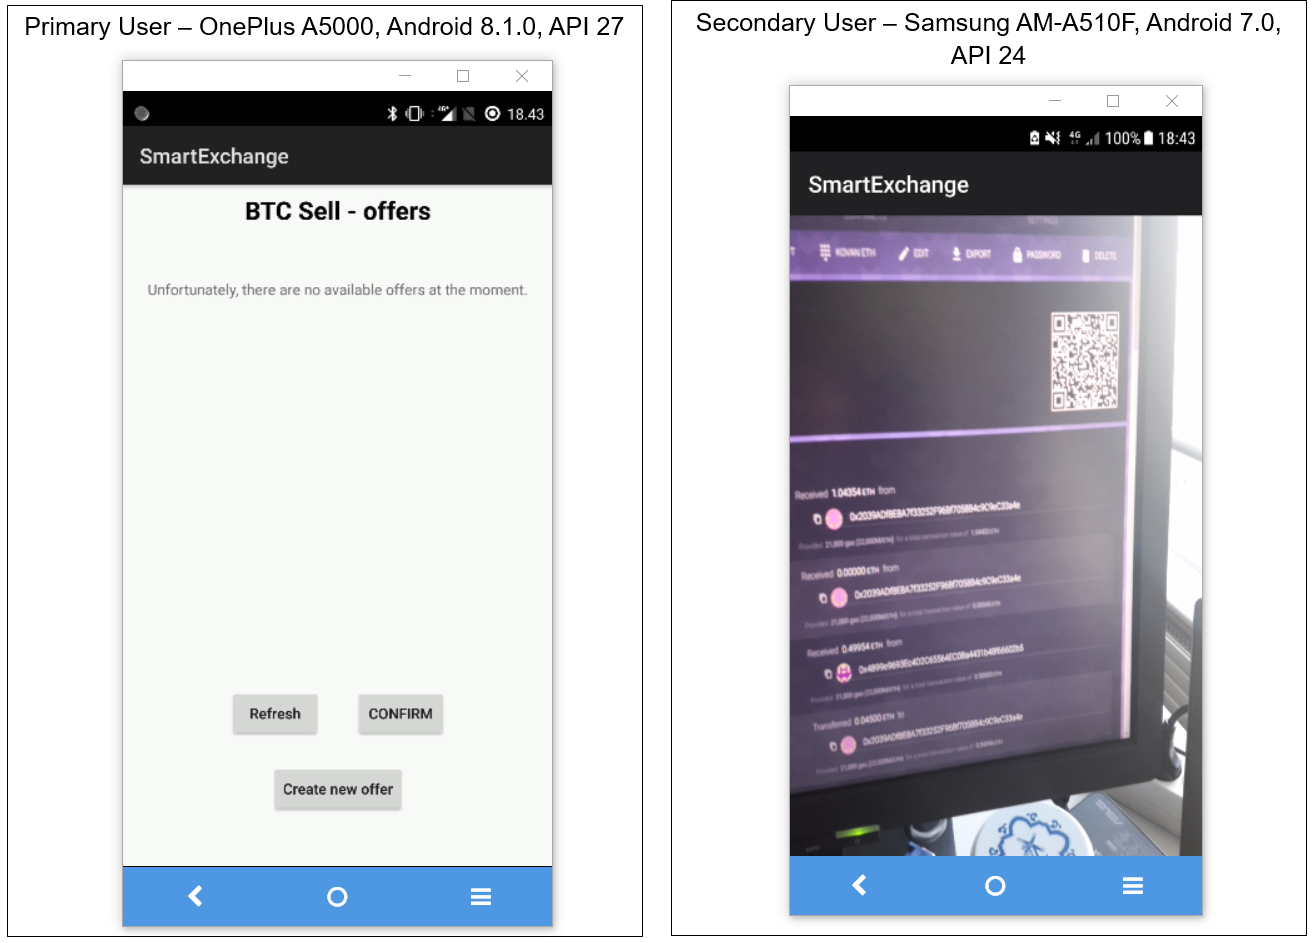
\includegraphics[width=0.85\textwidth]{screenshots/screen033}}
    \textit{Top:}    The secondary user filled in the details of the Bitcoin offer.\\
    \textit{Bottom:} The secondary user clicked on \textit{OR} button to scan the destination Ethereum address.\\
    \centerline{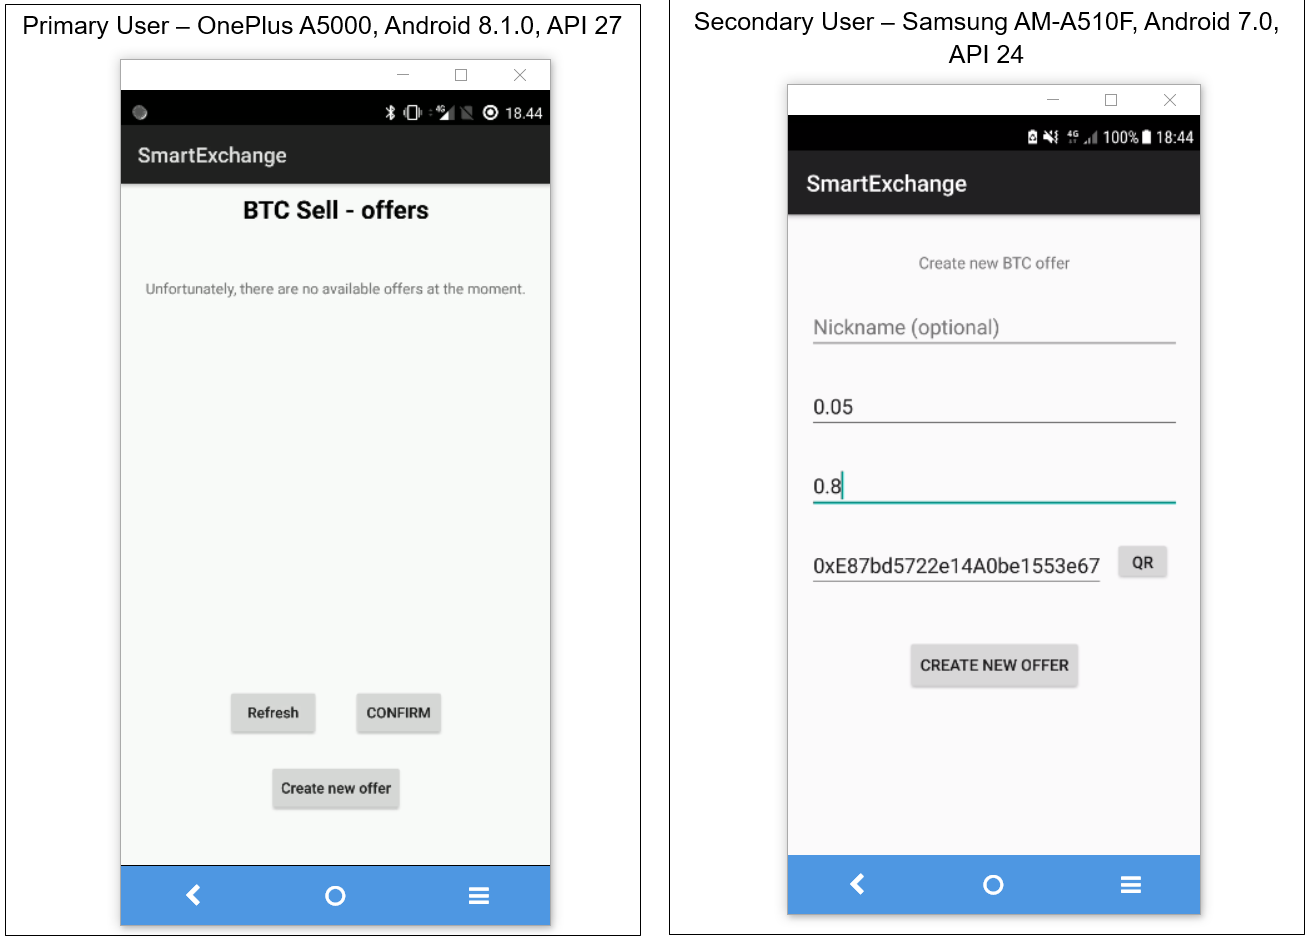
\includegraphics[width=0.85\textwidth]{screenshots/screen034}}
    \centerline{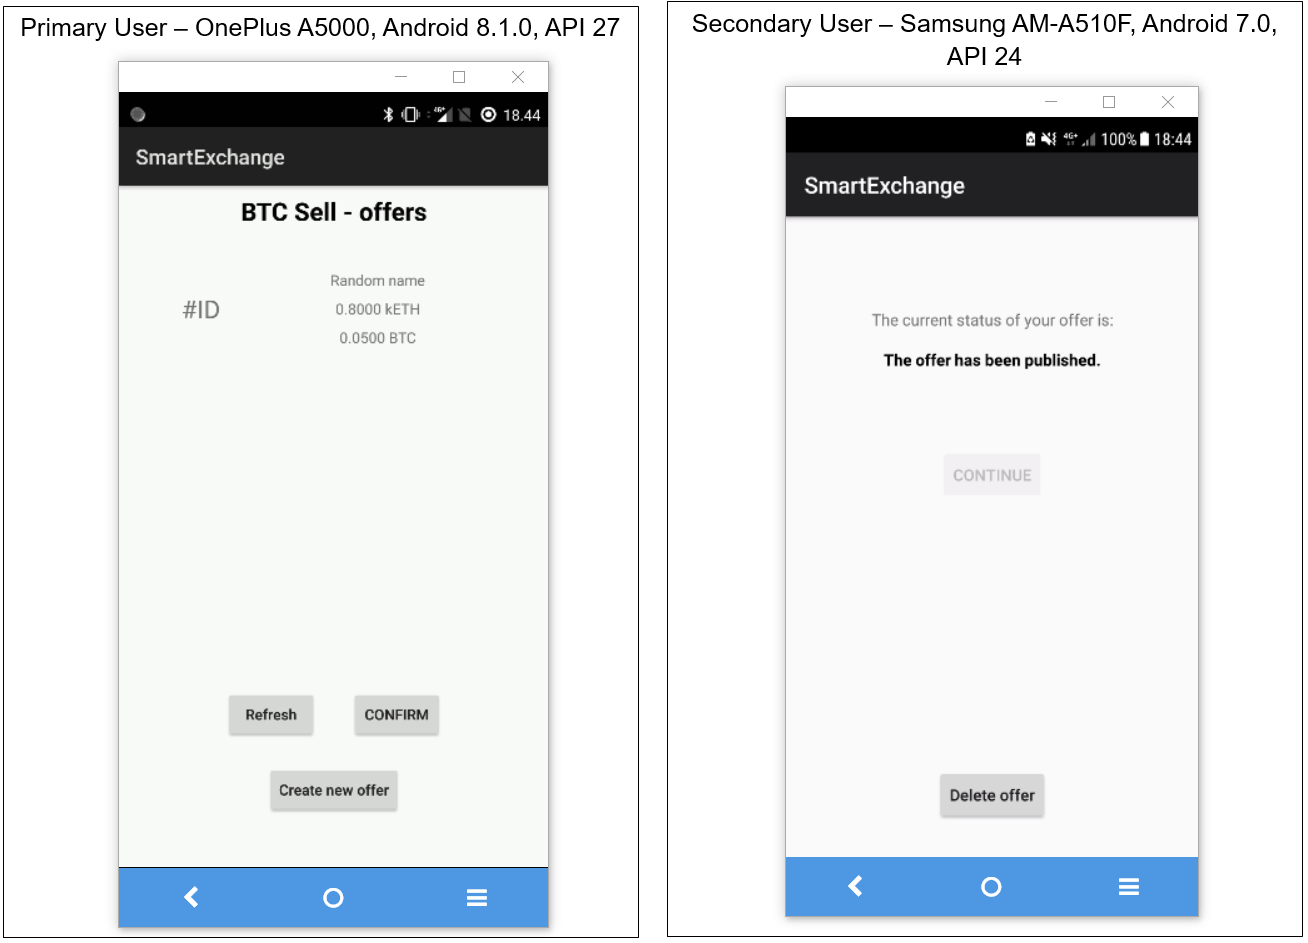
\includegraphics[width=0.85\textwidth]{screenshots/screen041}}
    \textit{Top:}    The Ethereum address was filled by the QR code scan.\\
    \textit{Bottom:} The secondary user clicked on \textit{Create new offer}.\\
    \centerline{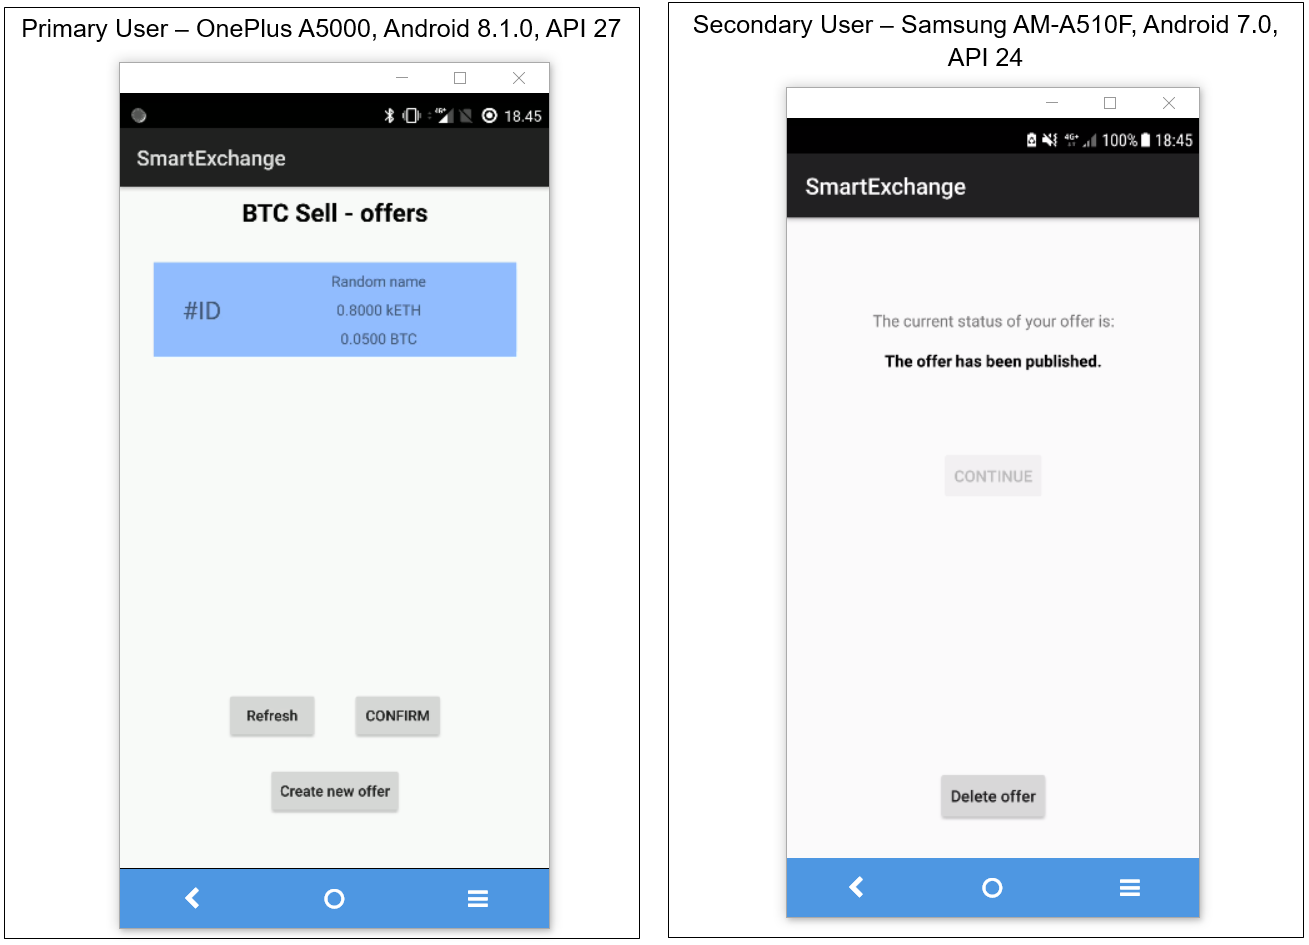
\includegraphics[width=0.85\textwidth]{screenshots/screen042}}
    \centerline{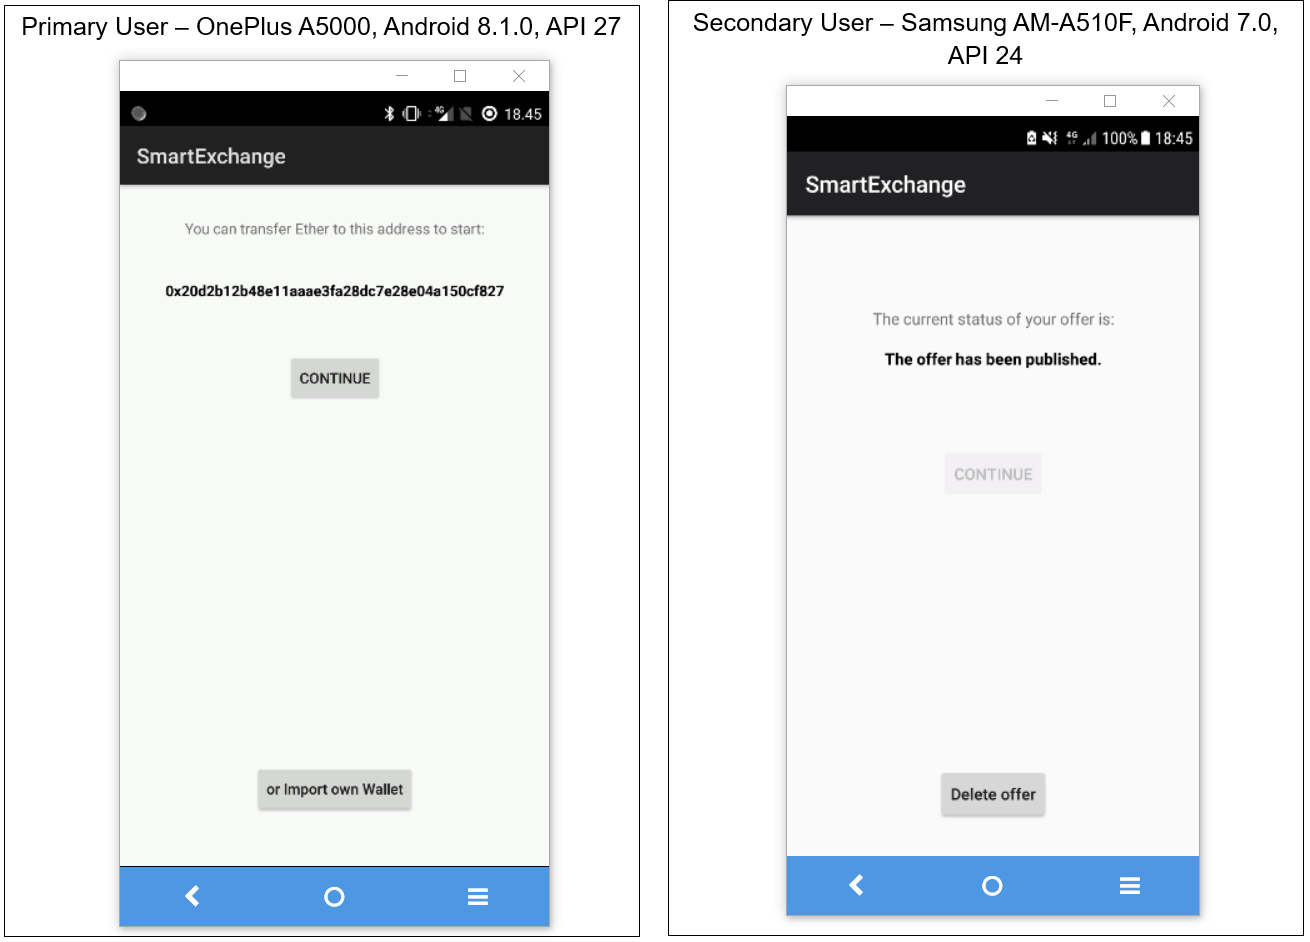
\includegraphics[width=0.85\textwidth]{screenshots/screen043}}
    \textit{Top:}    The primary user selected the offer from the list.\\
    \textit{Bottom:} The primary user clicked on \textit{Continue}. A screen prompting them to transfer funds to said Ethereum address was displayed.\\
    \centerline{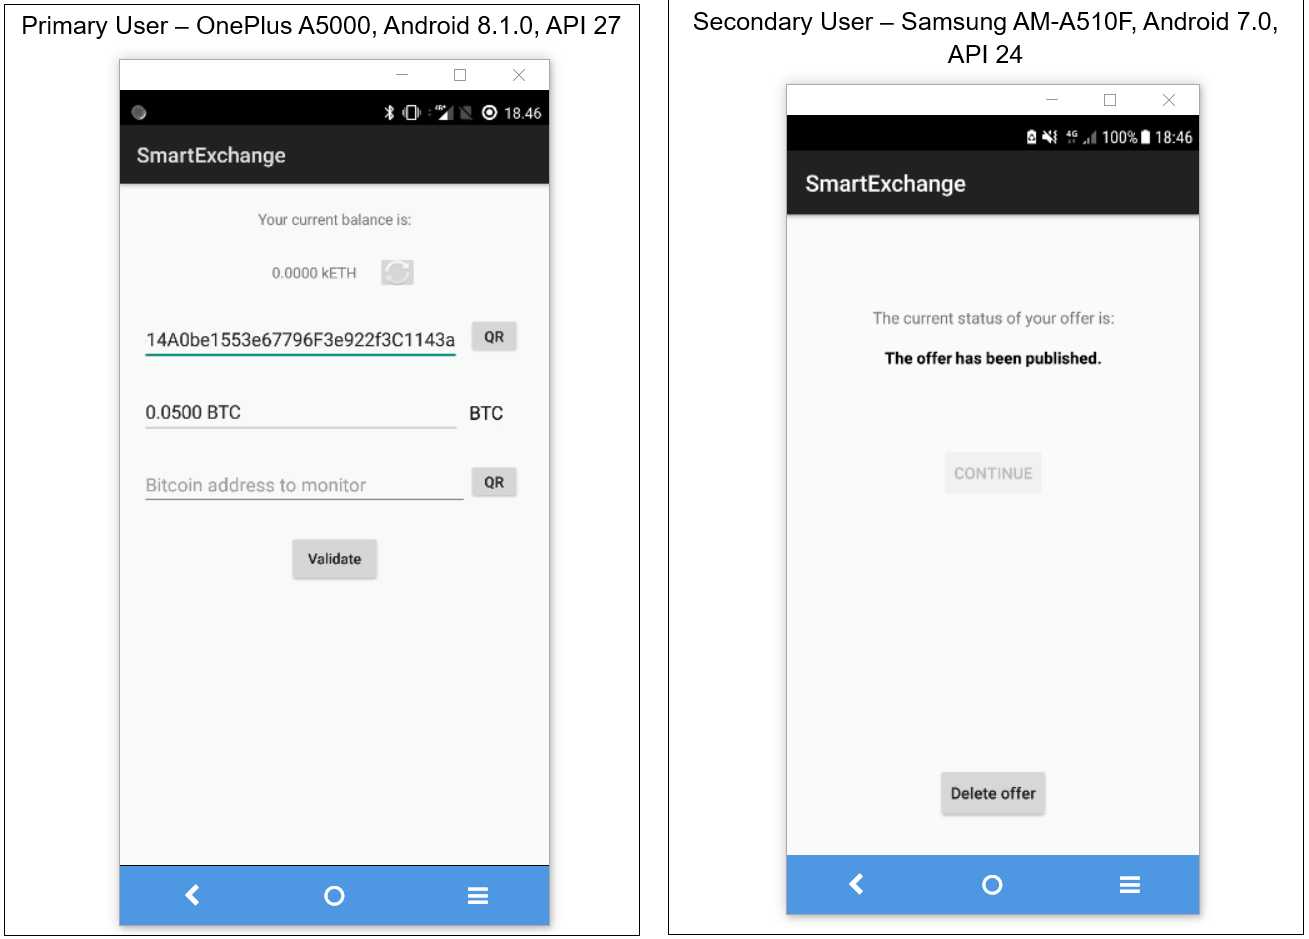
\includegraphics[width=0.85\textwidth]{screenshots/screen051}}
    The primary user clicked on \textit{Continue}. A screen prompting them to fill in their Bitcoin address was displayed. The Ethereum address and Bitcoin address are pre-filled.\\
    \centerline{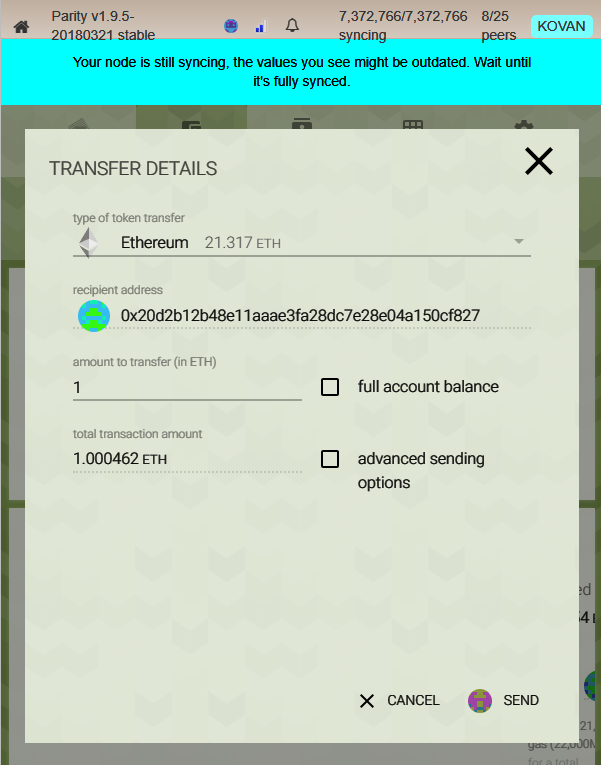
\includegraphics[width=0.85\textwidth]{screenshots/screen060}}
    The primary user deposited Ether to the temporary Ethereum address.\\
    \centerline{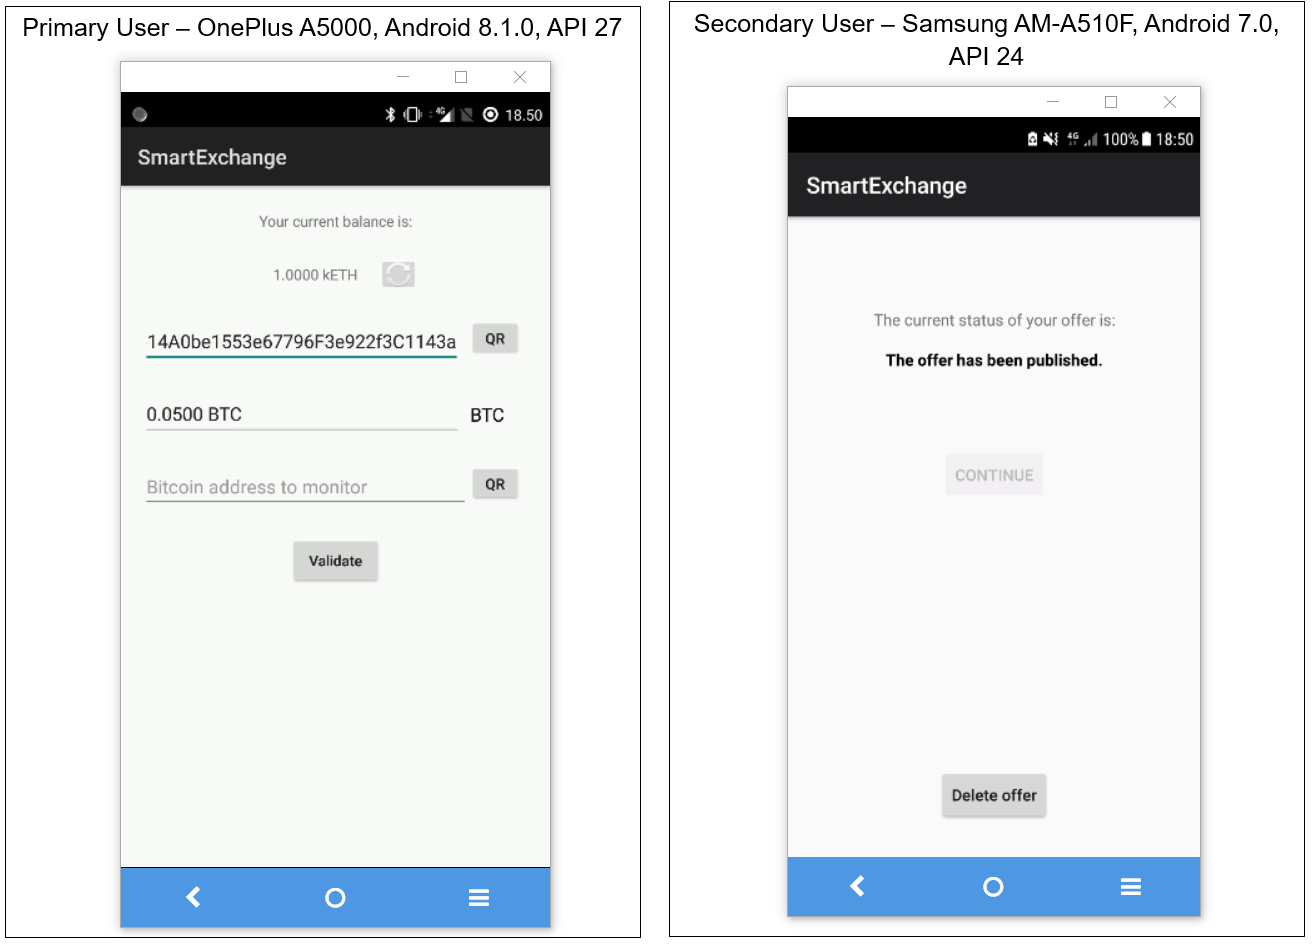
\includegraphics[width=0.85\textwidth]{screenshots/screen071}}
    \centerline{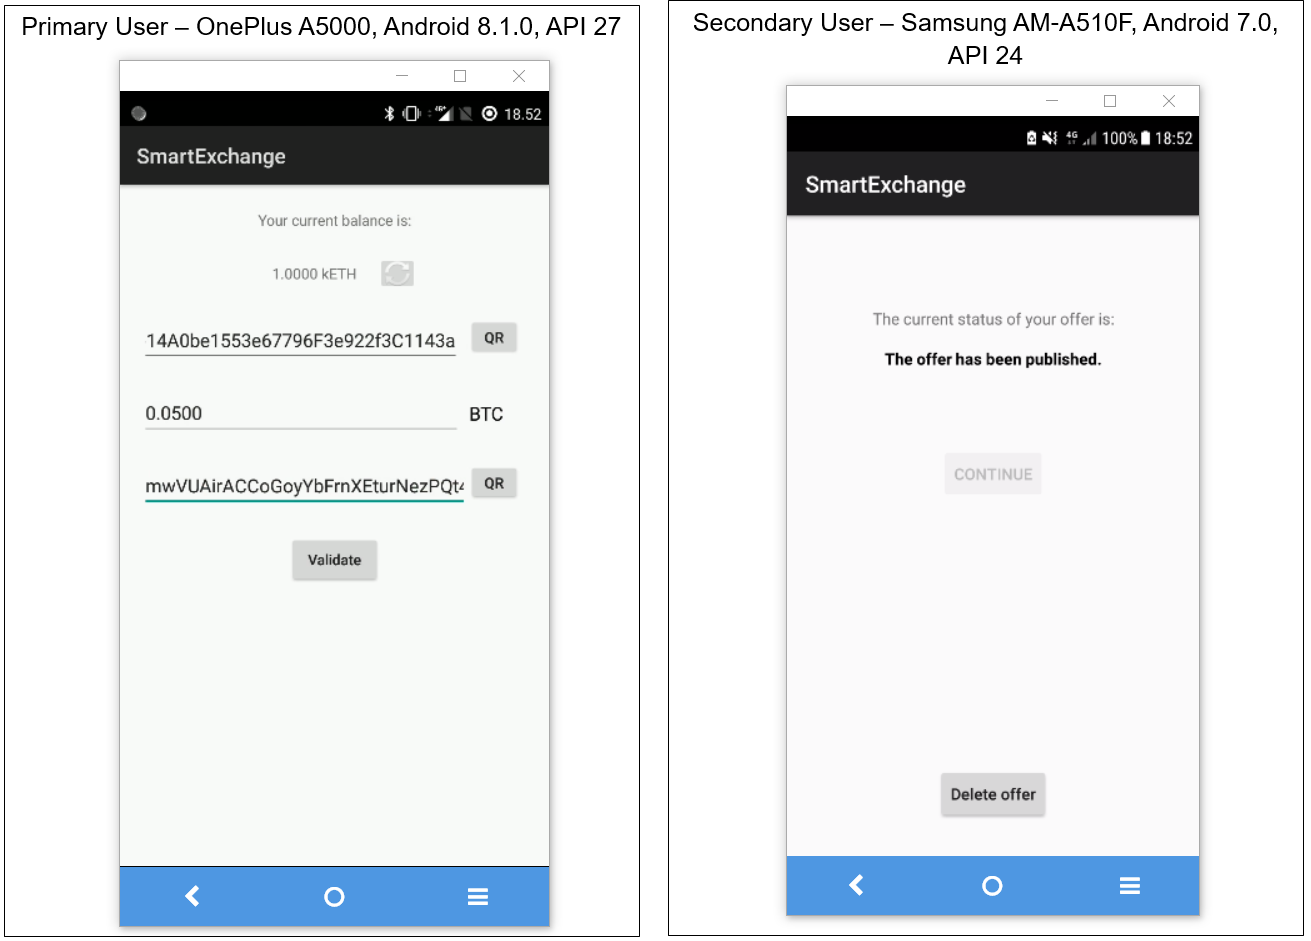
\includegraphics[width=0.85\textwidth]{screenshots/screen072}}
    \textit{Top:}    The balance of the temporary Ether wallet has changed.\\
    \textit{Bottom:} The primary user filled in their Bitcoin address.\\
    \centerline{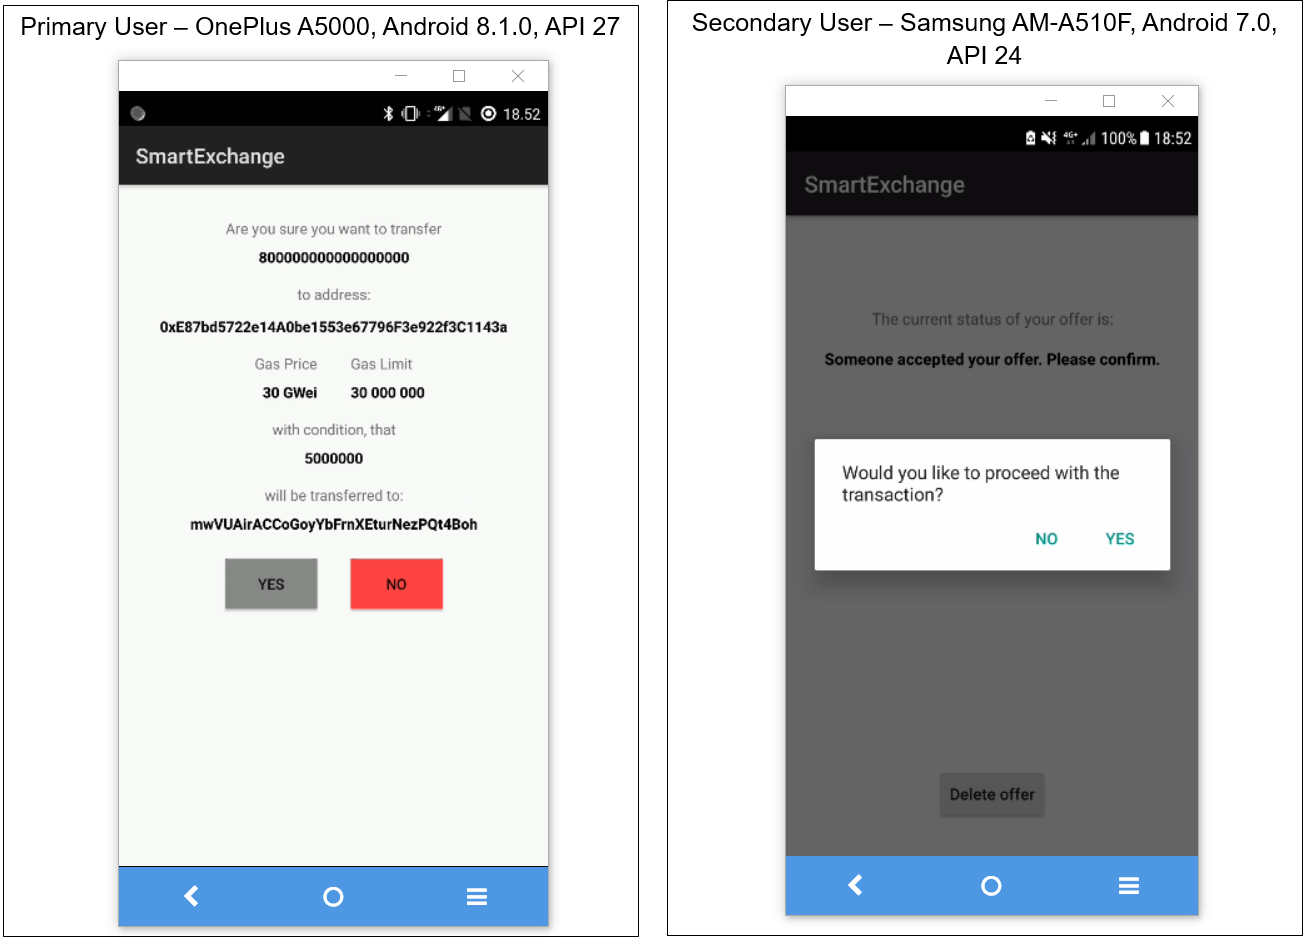
\includegraphics[width=0.80\textwidth]{screenshots/screen081}}
    \centerline{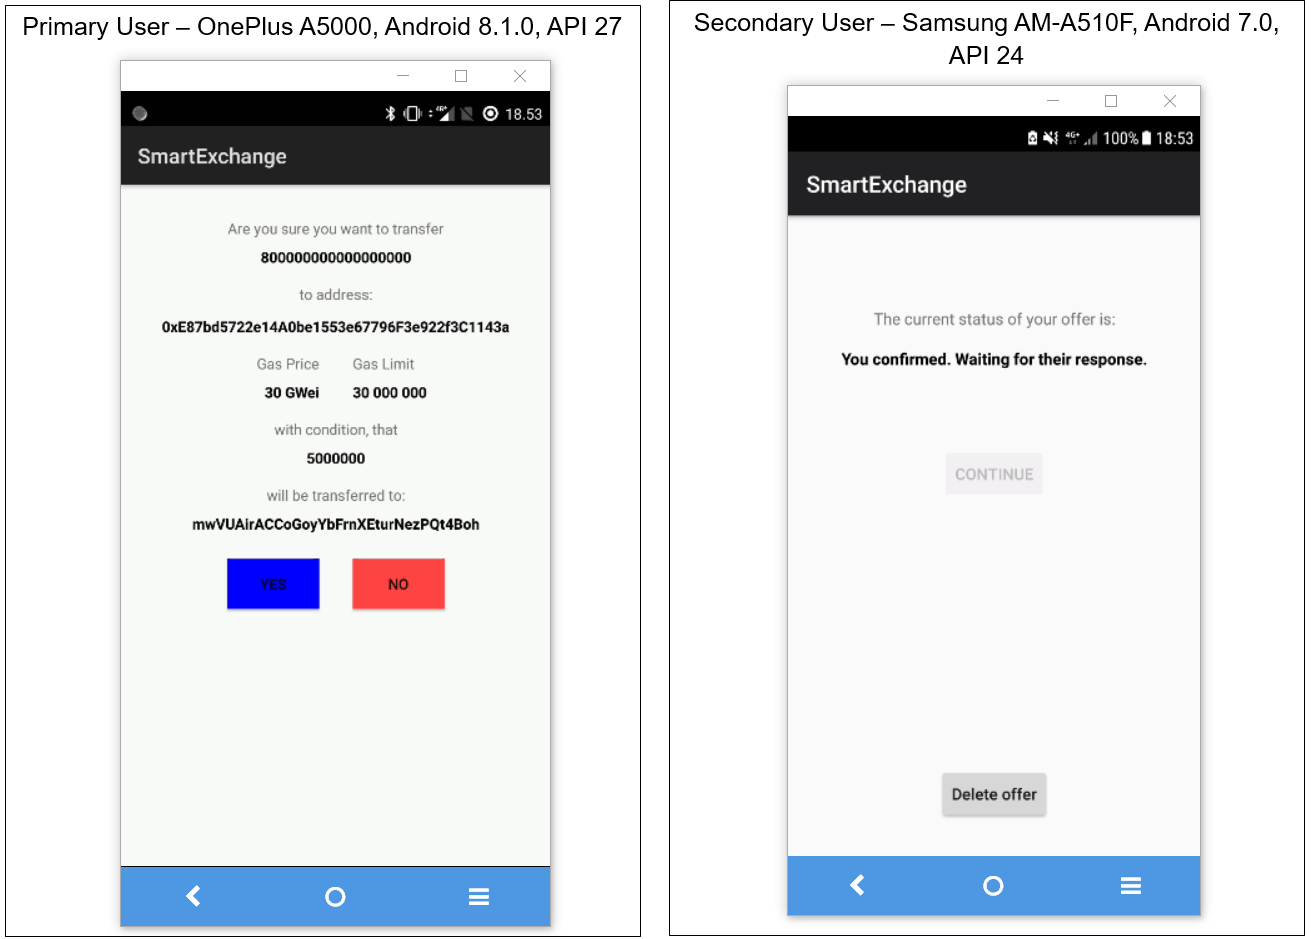
\includegraphics[width=0.80\textwidth]{screenshots/screen082}}
    \textit{Top:}    The primary user clicked on \textit{Validate}. This displayed a validation screen and triggered a prompt at the secondary user's device.\\
    \textit{Bottom:} Secondary user pressed \textit{Yes}. This action changed the colour of the \textit{Yes} button on primary user's screen.\\
    \centerline{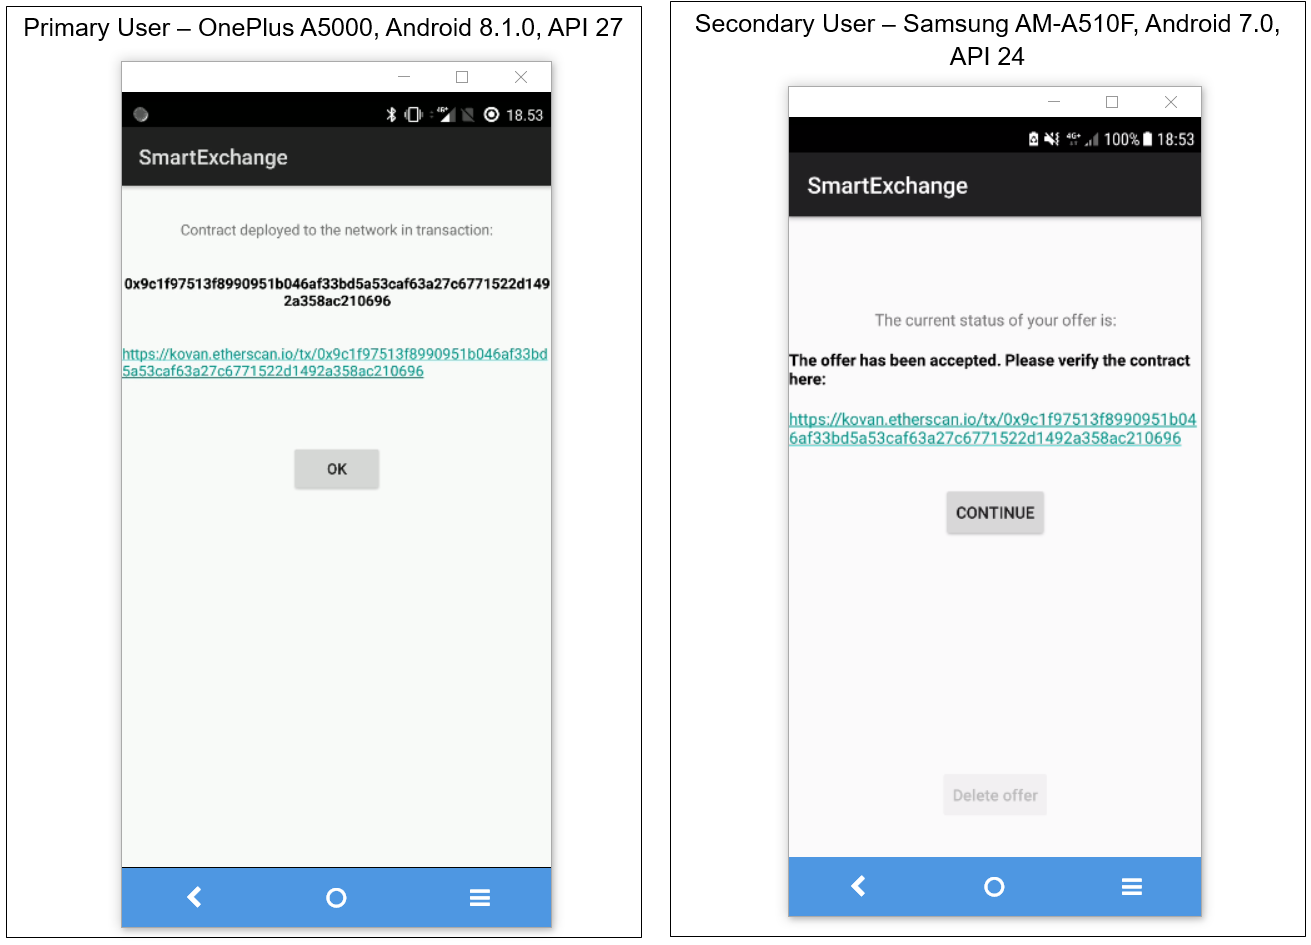
\includegraphics[width=0.80\textwidth]{screenshots/screen091}}
    \centerline{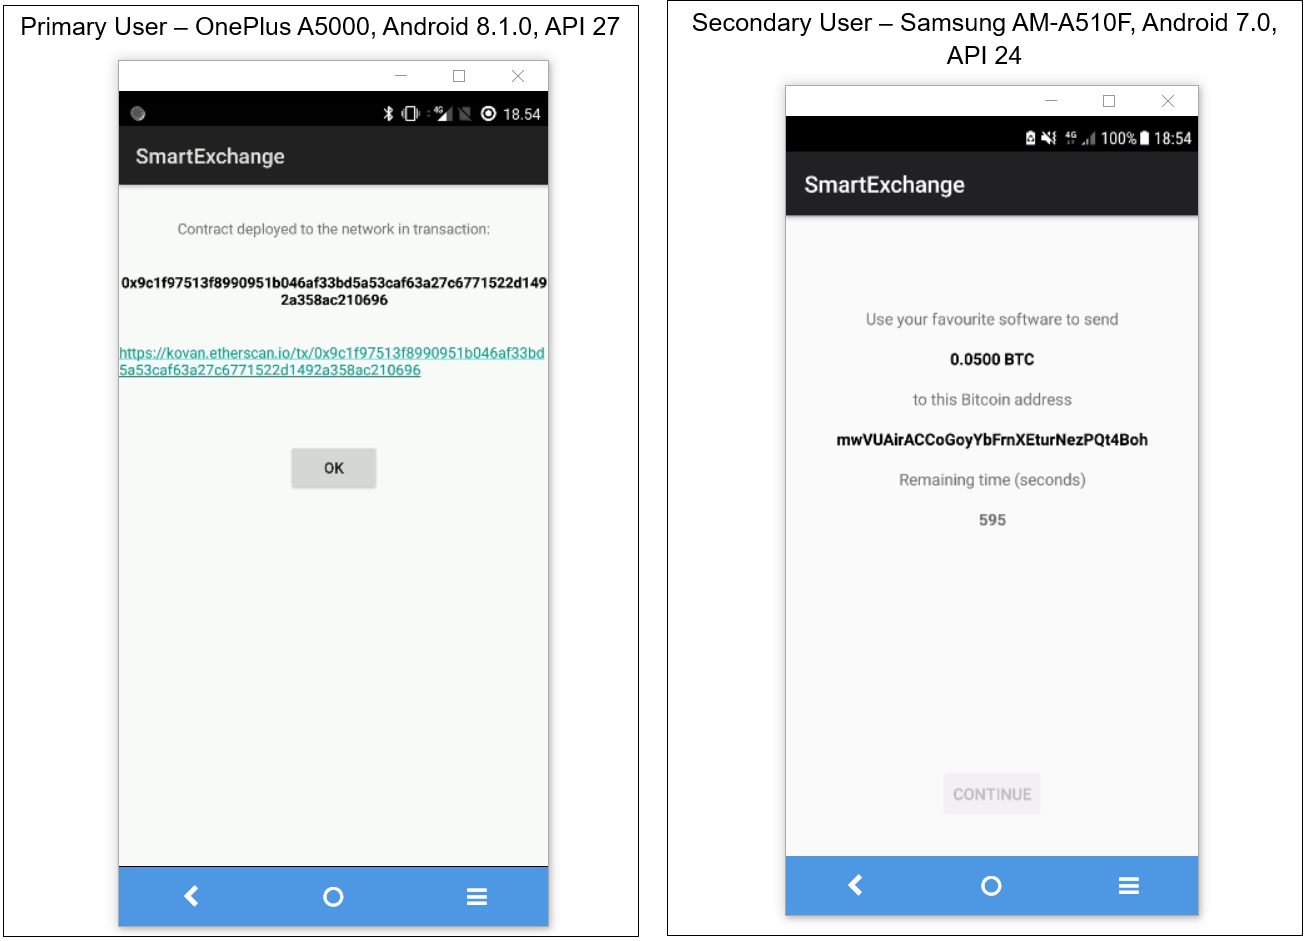
\includegraphics[width=0.80\textwidth]{screenshots/screen092}}
    \textit{Top:}    A transaction hash was displayed to the primary user and a link to blockchain explorer was displayed to both users.\\
    \textit{Bottom:} The secondary user clicked on \textit{Continue}. This displayed a screen, prompting them to transfer the Bitcoin\\    
    \centerline{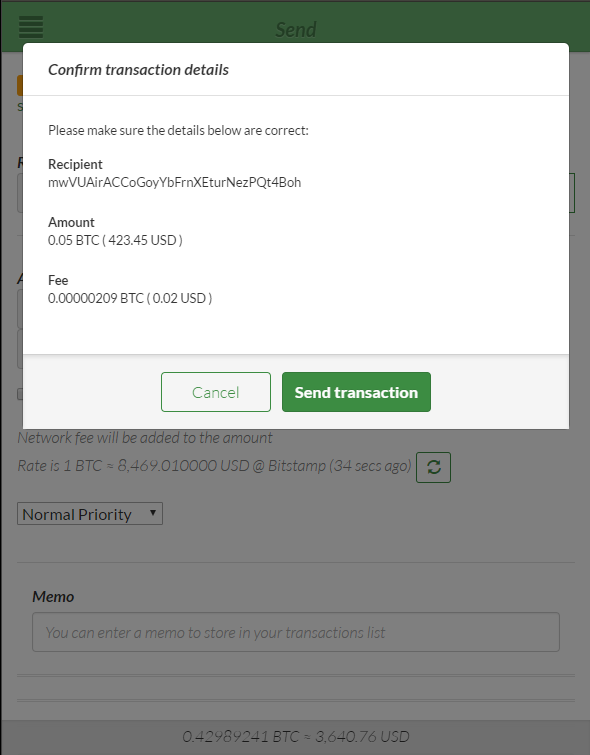
\includegraphics[width=0.85\textwidth]{screenshots/screen100}}
    The secondary user transferred the Bitcoin to the primary user.\\
    \centerline{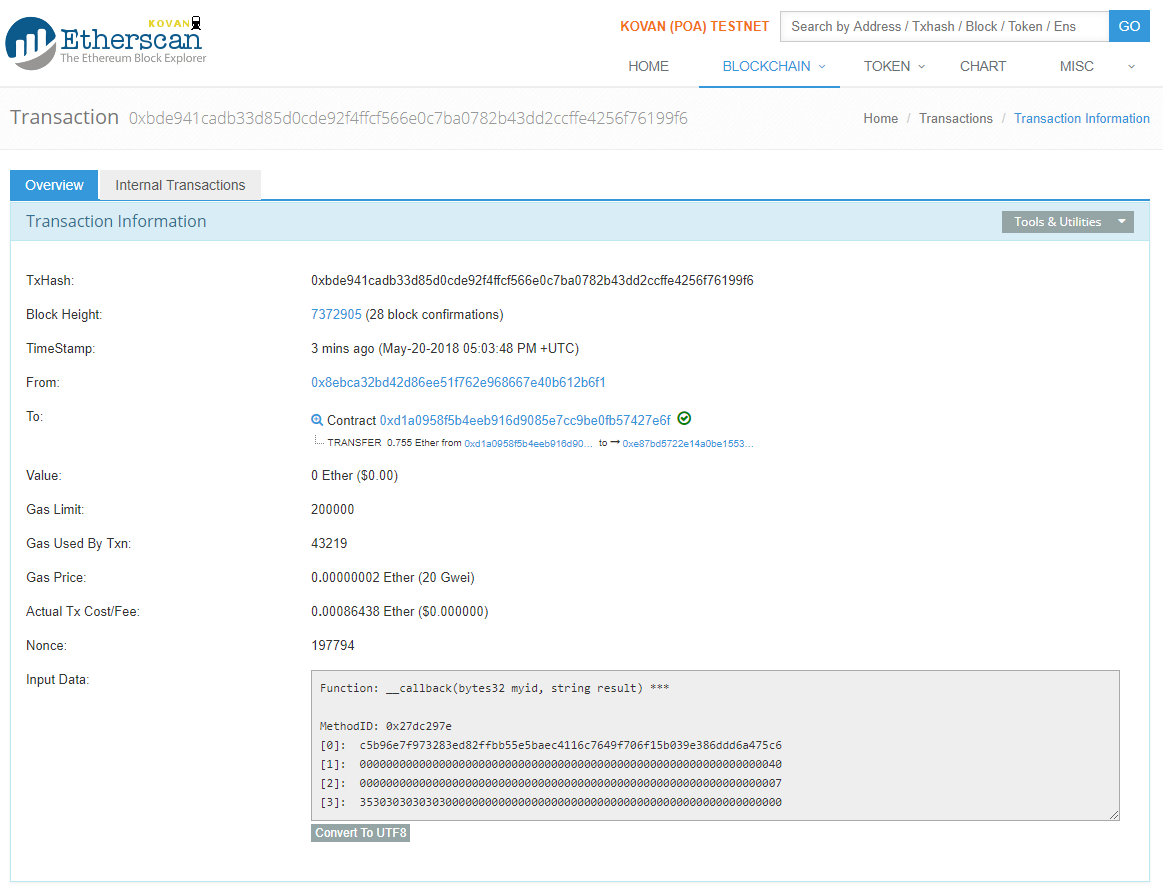
\includegraphics[width=0.85\textwidth]{screenshots/screen110}}
    The secondary user received their Ether.
    
